% Chapter 1

\chapter{Analysis of the State of the Art} % Main chapter title

\label{Chapter2} % For referencing the chapter elsewhere, use \ref{Chapter1} 

\lhead{Chapter 2. \emph{Analysis of the state of the art}} % This is for the header on each page - perhaps a shortened title

%----------------------------------------------------------------------------------------

\noindent In this section we discuss current research and solutions in the area of cloud applications' provisioning, deployment and management. Plenty of tools and approaches have been developed to address specific challenges in the management of the life-cycle of cloud applications, so the following analysis includes overview of the tools widely used by the industry players for the applications' provisioning and deployment, as well as findings from the latest research in this area. The analysis will lead us to the selection of the tool or approach on which we will focus our research efforts. To make a final selection, first we define a set of requirements which a given approach shall fulfill to be considered as a candidate for improvement. Then, we compare each discussed approach against our set of requirements and identify the final candidate. 

%----------------------------------------------------------------------------------------

\section{Requirements}

\noindent We analyze three areas of applications' provisioning, deployment and management to define our requirements, namely: provisioning and deployment process execution, workflow definition and topology description languages, and runtime application management. Essential requirements were defined in the research questions: the approach must be declarative (R1), open-source (R2) and provide support for continuous deployment (R3).

\noindent 

\noindent \textbf{Provisioning and deployment process execution.}

\noindent We have already discussed declarative and imperative approaches separately and their pros and cons in Section 1. Some tools can offer a mixture of these approaches: deployment workflow is derived from the application topology but the default order of operations and data exchange may be altered with the help of additional custom-written workflows, tasks or by setting of some specific properties in your application topology model \cite{juve2011automating, Breitenbuecher2014}. Tuning the order of operations and data exchange is definitely a useful feature (R4) and ideally it shall be possible to do this via some graphical tool, without writing any additional workflows, or at least with some high-level API. One more aspect here - some approaches install additional software on virtual machines during the deployment phase that may be used for monitoring or software installation. From the user perspective, it is better to avoid any additional software on every virtual machine because the application owner has to pay for the storage, CPU and RAM resources and it may affect the performance of the application. So, another requirement is that approach must be non-invasive: no additional software that is not directly related to the application on virtual machines (R5). Declarative approach requirement (R1) also falls into this category.

\noindent 

\noindent \textbf{Workflow definition and topology description languages.}

\noindent Topology description languages are mostly used in declarative approaches to describe the structure and final state of the cloud application, while workflow definition languages are used in imperative approaches for specifying each step of the deployment plan and their ordering. When we describe the topology of the application we usually think about virtual machines, databases, web servers and other application components. Nevertheless, some tools allow users to compose only virtual machines in their application topology model \cite{juve2011automating, konstantinou2009architecture}. We believe this is not sufficient because then application developers can enforce only the order of the virtual machines' provisioning and do not have any control over the ordering of the software installation and configuration. Such limitation reduces the flexibility of the given approach, so the ability to model full deployment stack (infrastructure, platform and services) by means of the topology description language is important too (R6). In Section 1 we mentioned that imperative approaches often rely on generic workflow definition languages, while offering a language specific to the domain of cloud deployment and provisioning would be more appropriate (R7) as we deal with concrete phases of the cloud applications' life-cycle. 

\noindent 

\noindent \textbf{Run-time application management.}

\noindent Challenges of the run-time applications management such as software updates, scaling, dynamic reconfiguration were discussed in Section 1. From that discussion we came up with requirement about continuous deployment that is related to dynamic reconfiguration of applications. Dynamic reconfiguration includes activities such as scaling and software updates, but in order to better distinguish one approach from another we put an ability to scale applications components as a separate requirement (R8). Last but not least, as we discussed earlier, dynamic reconfiguration may be achieved in several ways and one efficient way to implement it, is by calculating the difference between the running system and a new version of it and then applying only commands related to this difference (R9).

\noindent 

\noindent \textbf{Cross-cutting requirements.}

\noindent Again, following the arguments from the Section 1, all previously mentioned challenges become more complex when application owners want to use multiple cloud providers at the same time for different parts of their application. Such scenario affects all deployment phases and as an example, we may consider application scaling: on a single cloud it means increasing capacity of the server or adding more servers to the same cloud, while in multi-cloud environments we would refer to what is called cloud bursting \cite{amedro2010efficient} -- a situation when there is sudden increase in computation requirements and some resources from the user's local environment or private cloud are offloaded to another cloud provider. This may happen because application providers do not have enough capacity on their private cloud or because increase in computations affects performance of business critical modules of the application, so non-business critical components will be moved to another cloud. Nevertheless, nowadays multi-cloud deployments are essential to avoid vendor lock-in (R10). Another listed challenge was provisioning of resources on IaaS and PaaS levels simultaneously (R11). Open-source requirement (R2) also belongs to the additional requirements category as it does not affect the deployment process anyhow.

\noindent 

\noindent Based on these areas of interest, here is our grouped list of requirements:

\noindent 

\begin{enumerate}
\item  Provisioning and deployment process execution:
\begin{enumerate}
\item  R1 - ``Declarative approach'': provisioning and deployment workflow (plan) must be derived from the application topology model.

\item  R4 - ``Workflow refinement'': it must be possible to change derived workflow at least in terms of the order of operations and data exchange.

\item  R5 - ``Non-invasive'': no additional software (software that you did not define as part of your application) shall be installed on virtual machines to facilitate the application deployment.
\end{enumerate}

\item  Workflow definition and topology description languages:

\begin{enumerate}
\item  R6 - ``Full deployment stack modelling'': it must be possible in the application topology model to describe any types of application components like virtual machines, servers, relationships to allow specification of dependencies on different levels, not only between virtual machines. 

\item  R7 - ``Domain-specific workflow definition language'': the workflow definition language must reflect tasks and behaviors relevant to the area of provisioning and deployment of cloud applications.
\end{enumerate}

\item  Run-time application management:

\begin{enumerate}
\item  R8 - ``Scalability'': it must be possible to scale application components in and out either via API/CLI calls, or topology description updates, or policies.

\item  R3 - ``Dynamic reconfiguration'': it must be possible to reconfigure application during the run-time and update the application topology model or deployment plan according to the new application state.

\item  R9 -- ``Efficient reconfiguration'': dynamic reconfiguration of the application must be performed by applying the necessary modifications to the running system instead of redeploying the whole application. In addition, it is important that the application owner has an overview of the running system, so he can be sure which changes to make. This is essential because components may fail and the system may not be identical to the one that was defined during the design-time, so applying changes to such system will result in the wrong state of the application.
\end{enumerate}

\item  Cross-cutting requirements:

\begin{enumerate}
\item  R10 - ``Multi-cloud'': ``Multiple Cloud delivery model assuming no prior agreement between the Cloud providers and a third party responsible for provider contracting, consumption negotiation, SLA monitoring, inter-provider networking, code and data migration'' \cite{petcu2014consuming}. Although, in our case we do not consider data migration and synchronization.

\item  R11 - ``IaaS and PaaS resources provisioning'': it must be possible to provision resources on different levels of the cloud computing stack.

\item  R2 - ``Open-source''\footnote{ The Open Source Initiative, $  $http://opensource.org/osd}: the code of the project must be freely accessible for use and modification.
\end{enumerate}
\end{enumerate}

%----------------------------------------------------------------------------------------

\section{Tools and Approaches}

\noindent The above set of requirements allows us to start the analysis of different tools and approaches for the provisioning and deployment of cloud applications.

\noindent Some approaches operate only on one level of the cloud stack, for example, they manage dependencies only between virtual machines or between middleware components. Example of such approaches are presented in \cite{juniormodel, konstantinou2009architecture} and \cite{juve2011automating}. 

\noindent In \cite{juniormodel} an automatic model-based approach to software deployment is proposed. It is a declarative approach. The deployment process is derived from UML models based on dependencies between so-called services (components), not virtual machines. One UML model is general and includes application topology view, and another one is provider-specific - includes the name of the provider and credentials. Deployment is performed with a help of 14BIS (a platform to deploy third party software) as a software repository and Chef\footnote{ Chef automation tool, https://www.chef.io/}. During the deployment, a list of recipes (installation scripts) is uploaded to each virtual machine and executed there. This approach is provider independent in terms of infrastructure providers, but it is tied to the deployment service provider - 14BIS platform. Developers can define application topology~and it will be properly deployed, but they can not tune the order of the deployment - a major limitation of declarative approaches. In addition, this approach has no functionality for the run-time phase and no code available for testing purposes, and it is invasive because of usage of Chef.

\noindent 

\noindent The approach presented in\cite{ konstantinou2009architecture} consists of three models: (i) virtual solution model (VSM), which is a set of composable virtual appliance models (virtual images with pre-built configuration points); (ii) VSM is transformed into the virtual solution deployment model (VSDM) that can have some additional cloud-specific properties; (iii) a VSDM is then transformed into virtual solution deployment plan (VSDP) which is responsible for the cloud application provisioning and deployment (Figure \ref{fig:virtual}). 

\begin{figure}[htbp]
	\centering
		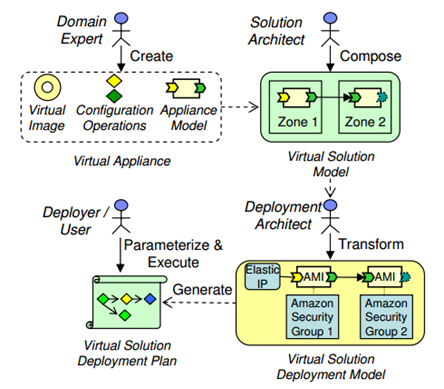
\includegraphics{./Figures/Konstantin}
		\rule{38em}{0.5pt}
	\caption[Virtual Solution Approach]{Virtual Solution Design and Deployment}
	\label{fig:virtual}
\end{figure}

\noindent A few limitations of this approach are: every model must be configured manually by expert users, the only available implementation is proprietary and application topology model (VSM) is based on the composition of pre-built virtual machines, not on the independent software components. Regarding the deployment - details are not covered in the paper but it is based on the research of the deployment patterns and constraints on virtual machine' ports: linkage of ports implies a deploy order dependency. The actual deployment plan is performed by platform-specific workflows (for instance, IBM Solution Assembly Toolkit workflow or Eclipse job manager). So, this is a declarative approach to some extent (Virtual Appliance and Virtual Solution Model), but it requires a lot of human involvement to prepare VMs and all models, and it has the same problem as the previous approach - deployment order can not be changed after VSM is ready. 

\noindent 

\noindent In \cite{juve2011automating} a multi-cloud solution called Wrangler is described. Application topology is described there using specific XML dialect. A topology description is sent to the WRANGLER web-service (multiple interfaces are available: XML-RPC, Python API, command line) which orchestrates provisioning and deployment of the application. Each component may have a bunch of plugins (scripts) which are used for its configuration. The deployment order is decided from DAG-based\footnote{ Directed Acyclic Graph, http://en.wikipedia.org/wiki/Directed\_acyclic\_graph} dependencies in XML document and component groups. Dependencies define the order of VM's provisioning and configuration, and groups are used for systems that require nodes to know about each other. First, all VMs of a group are provisioned (so their IP is known and may be shared with other nodes) and only after that configured. This approach may be attractive because deployment to multiple clouds at the same time is possible, and some run-time commands are available like adding or deleting nodes (no dynamic reconfiguration is possible), and also monitoring of VMs can be done. Nevertheless, it supports only IaaS-level dependencies between components, no code or implementation is available, plugins must conform to a standard set of operations (start, stop, status), serial provisioning of VMs, and this approach is invasive - you have to prepare VMs by installing some additional software before you can use them as part of the topology.

\noindent 

\noindent More advanced approaches allow application developers to define application components and their relationships on all three cloud stack levels (IaaS, PaaS and SaaS) and in addition, they usually allow deployments to multiple clouds simultaneously (although WRANGLER, which was mentioned before, also has such capability) and have more advanced operations for the run-time management (for example, policy-based application management). Two of such approaches are TOSCA and Apache Brooklyn.  

\noindent 

\noindent TOSCA \cite{INPROC-2013-45} application topologies can be processed in an imperative or declarative way. Imperative processing relies on management/build plans (workflows) which are typically implemented by the application developer. Plans define required services in an abstract way, concrete endpoints are bound from implementation artifacts (e.g., SOAP Web services, REST, scripts) of application components (nodes). Plan Portability API allows access to topology and instance information, for instance, property values of nodes and relationships (runtime info: ports, IP of VMs). Credentials and configurations (for instance, machine size) are passed to the Build Plan as inputs. During the run-time, the workflow engine enacts operations of the build plan and in that way the application is provisioned and deployed. Dynamic reconfiguration may be theoretically achieved by writing new plans and running them on top of the existing application, but if many such plans will be written, eventually it will be not possible to maintain such application. Declarative processing of applications in TOSCA is possible with Plan Generator \cite{Breitenbuecher2014} which takes a topology with all artifacts (deployment and implementation) as input and produces fully executable workflow that can be adapted afterwards. Plan Generator was a separate tool at the time the paper was published and we were unable to find any more recent information about it. The order of the provisioning is based on the types of Relationship Templates: if node A is ``hostedOn'', ``dependsOn'', ``runsOn'' node B, then node B must be provisioned first. Relations of types ``calls'', ``invokes'', ``connectsTo'' require both nodes to be instantiated before the relation can be instantiated. In addition, TOSCA simple profile in YAML \cite{TOSCA-Simple-Profile-YAML-v1.0}is under development that will allow declarative provisioning and deployment, probably based on the repository of the node and relationship types. The main limitation of TOSCA is that it is not possible to dynamically reconfigure the application.

\noindent 

\noindent Another available system is Brooklyn\footnote{ Apache Brooklyn, $  $https://brooklyn.incubator.apache.org/} which is used for deploying and managing distributed applications. It is an open-source system, it supports multi-cloud deployments and also the definition of PaaS-level components in the application topology model. Application topology is described in YAML or JAVA blueprints via entities (pieces of code) which can have operations, attributes, policies and sensors (for monitoring). Run-time operations such as scaling are available, including monitoring and policy-based management of the application. The deployment order is based on the hierarchical tree of entities (each entity has a parent and may have children, except application entity that is a top-level entity) and is done in parallel. Default provisioning order may be customized with the help of tasks if the user needs to defer the start of one entity before another one reaches some state and can share its values for instance. The deployment execution status is visible to operators. A repository of entities is available which makes it easier to construct applications. Limitations of the approach include: (i) it is not possible to change topology (and thus deployment order) with regard to the underlying schema (parent-child relationships) and (ii) it is not possible to dynamically reconfigure the application.

\noindent 

\noindent Next stage of the improvement to deployment processes brings the capability to update applications dynamically during their run-time. A few systems that have such feature are CloudMF, Cloudify and SmartFrog.

\noindent 

\noindent 

\noindent CloudMF consists of a cloud modelling DSL called CloudML which allows abstract description of the desired application topology along with the specification of its provisioning and deployment, and a models@run-time environment for the enactment of the provisioning, deployment and adaptation of the application. Models@run-time is a unique feature of CloudMF as authors state in their paper \cite{FerrySongRCS14}: ``.. the work of Shao \cite{ShaoWeiWM10} was a first attempt to build a models@run-time platform for the cloud, but remains restricted to monitoring, without providing support for configuration enactment. To the best of our knowledge, CloudMF is thus the first attempt to reconcile cloud management solutions with modeling practices through the use of models@run-time.'' Models@run-time environment provides the causal connection between the running system and application topology model. So, after the initial application was deployed, application owners can change the application topology model and issue a deploy command. After that the deployment engine will compute required changes and update the running application. Update in this case means only performing the necessary modifications such as the  deployment of new components thus, there is no need to redeploy the whole application. From the other side, if some VM crashes, this information will be automatically populated in the in-memory application topology model. The deployment order in the CloudMF is based on the engine policies and components' requirements and capabilities. For instance, a web server requires a database to operate properly, this means that the database will be installed and started before the web server. CloudMF is also a declarative approach, so it is not possible to tune the deployment order to the user's specific needs. In addition, scalability functionality is not yet implemented properly: if it is required to create one hundred VMs of the same type, the developer will need to describe each of them. In addition, deployment tasks are executed sequentially, which is not suitable for large-scale applications deployment. The project is open-source and the code is available on Github\footnote{ CloudML, https://github.com/SINTEF-9012/cloudml}.

\noindent 

\noindent Another similar tool called Cloudify\footnote{ Cloudify, $  $http://getcloudify.org/} focuses on cloud orchestration and automation. A topology is described in a blueprint that is inspired by the TOSCA YAML profile and includes application nodes, workflows and relationships. From blueprints, developers can create deployments (i.e., blueprints enriched with input data), and then run built-in or custom workflows to deploy or undeploy the application. Provisioning and deployment are done with the help of a stateful orchestrator called Manager that runs automation processes described in workflows. Each task of the workflow is delegated to Agents: manager side agents are responsible for the provisioning, and application side agents - for the deployment of different components. Finally, the actual execution of each task is performed with the help of Plugins: scripts, Chef, Puppet or Docker tools. Regarding the order of execution, default order is based on relationships of nodes (all nodes may be started in parallel) and built-in lifecycle of a node: create node, preconfigure relationship, configure node, post-configure relationship, start node, install agent workers and required plugins, establish relationship, start monitoring. Any node may have custom workflows that will change the default execution order. Multi-cloud support, a repository of blueprints and some plugins are available only in premium version what makes this approach less attractive for the users. Regarding the dynamic reconfiguration capabilities of the Cloudify -- in some places in the documentation and a few use cases that highlight the benefits of Cloudify, it can be found that such feature is available. At the same time, it is not clear what they mean by the dynamic reconfiguration (seems to focus mainly on the scaling of the application) and no details are provided about how exactly this can be done.

\noindent 

\noindent In\cite{Frog}, an extension to SmartFrog framework \cite{goldsack2009smartfrog} is presented which allows multi-cloud deployments and application adaptations during the run-time phase. Each application component is modeled as an object whose lifecycle events correspond to specific actions like Deploy, Start, and Terminate. The deployment manager can link the lifecycle of different components by such constructs as compound (start and terminate components together), parallel (start components concurrently and let them evolve independently) and sequence (a component start only after previous component terminated) and this linking will determine deployment plan. Later on, when some component has to be moved to another cloud for instance, deployment manager can query Metadata database to determine dependencies of this components, and based on the query result, adaptation is executed. Details are not clearly explained: in \cite{goldsack2009smartfrog} researchers simply mentioned that some programs must interact with SmartFrog framework to handle application adaptation scenarios. In addition, in \cite{Frog} two evaluation scenarios that were presented focused on migration of services from one cloud to another, so it seems like the dynamic reconfiguration is possible but only in terms of the changes to the location of services, not to the underlying services architecture. Other drawbacks of this approach are: each VM runs SmartFrog daemon, so the approach is invasive, and it is not possible to refine the workflow - deployment plan will be based on the chosen deployment construct (compound, parallel, sequence). 

%----------------------------------------------------------------------------------------

\section{Summary}

\noindent After analyzing each approach we summarize our findings in Table \ref{tab:1}. Requirements analysis was simplified to save some space in the descriptions of each approach, while Table \ref{tab:1} shows exactly how all approaches satisfy our list of requirements. Such requirements as ``Declarative approach'', ``Dynamic reconfiguration'' and ``Open-source'' were defined as essential requirements, so they are highlighted. ``N/A'' mark means that this requirement is not applicable to the given approach or there is no definite answer, for instance when some approach was not positioned as proprietary solution but at the same time we could not find a source code for it. ``yes*'' mark means that requirement is satisfied but under certain conditions. Finally, ``?'' mark refers to the situation when the approach claims to satisfy the requirement, but we could not find the information about how a given feature is implemented.

\noindent

\noindent Starting from the ``Declarative approach'' requirement we can see that all approaches satisfy this requirement, except TOSCA, which can offer declarative deployments with help of the Plan Generator as discussed before, but we were unable to get the code of the Plan Generator or to find its implementation. Next essential requirement is ``Dynamic reconfiguration'': only CloudMF, Cloudify and extended SmartFrog framework can provide such feature, so at this point five out of eight approaches can be eliminated. It is not clear what is meant by the dynamic reconfiguration in Cloudify and SmartFrog approaches: scaling of the application, relocation of virtual machines from one cloud provider to another, changing the parameters of some application components or changes to the application architecture, so they receive lower ranking than CloudMF with regard to the ``Dynamic Reconfiguration'' requirement. As for the ``Open-source'' requirement, all three approaches are open-source projects, but Cloudify offers such feature as multi-cloud deployments only under subscription, so we can eliminate it too. Between CloudMF and SmartFrog approaches we choose CloudMF because it is non-invasive and clearly satisfies such requirements as dynamic and efficient reconfigurations.

\begin{center}
	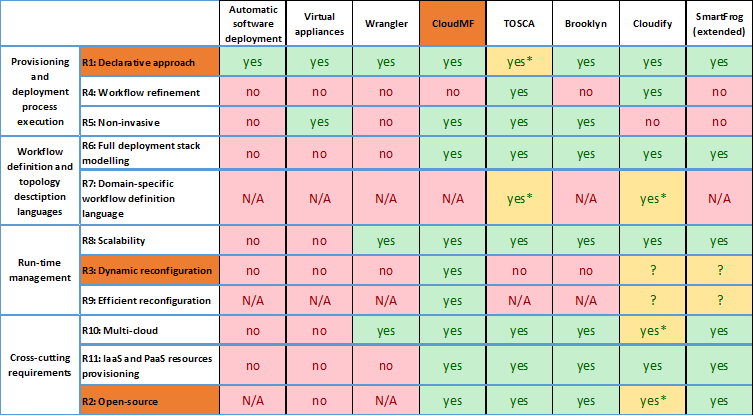
\includegraphics[width=38em]{./Figures/Comparison}
	\begin{table}[htbp]
    \caption{Comparison of Provisioning and Deployment Approaches}
    \label{tab:1}
	\end{table}
\end{center}


\noindent One more observation from the comparison is that there is no domain-specific language for provisioning and deployment of cloud applications. Cloudify relies on a so-called graph framework to specify custom workflows, but there is no details about it in the documentation right now, and looks like they went for such solution not because of some domain-specific semantics of the framework, but rather because it allows to parallelize tasks in an easy way through concrete API. As for TOSCA which currently uses BPEL for the definition of deployment plans, BPEL can be considered as domain-specific language for business process modelling, but not specific for the deployment domain. While it could be used in the deployment domain, if deployment actions were expressed as services, it seems too powerful and complex.